\begin{frame}
    \huge
    \misc{
        \textbf{Resultados}
    }
\end{frame}
\begin{frame}
    \misc{
        Se tiene la siguiente ecuación diferencial parcial:
        \begin{equation}
            \frac{\partial u}{\partial t} = \frac{\partial^2 u}{\partial x^2} \qquad 0<x<1, \; t>0 \label{eq:equation_1}
        \end{equation}
        con las siguientes condiciones de frontera:
        \begin{equation*}
            \begin{cases}
                u(x,0) & = sin(\pi x) \qquad 0<x<1 \\
                u(0,t) & =u(1,t) = 0, \qquad t>0
            \end{cases}
        \end{equation*}
        La solución análitica de este conjuntos de ecuaciones es:
        \begin{equation*}
            u(x,t)= e^{-\pi^2 t}sin(\pi x)
        \end{equation*}
    }
\end{frame}

\begin{frame}
    \begin{figure}[H]
        \centering
        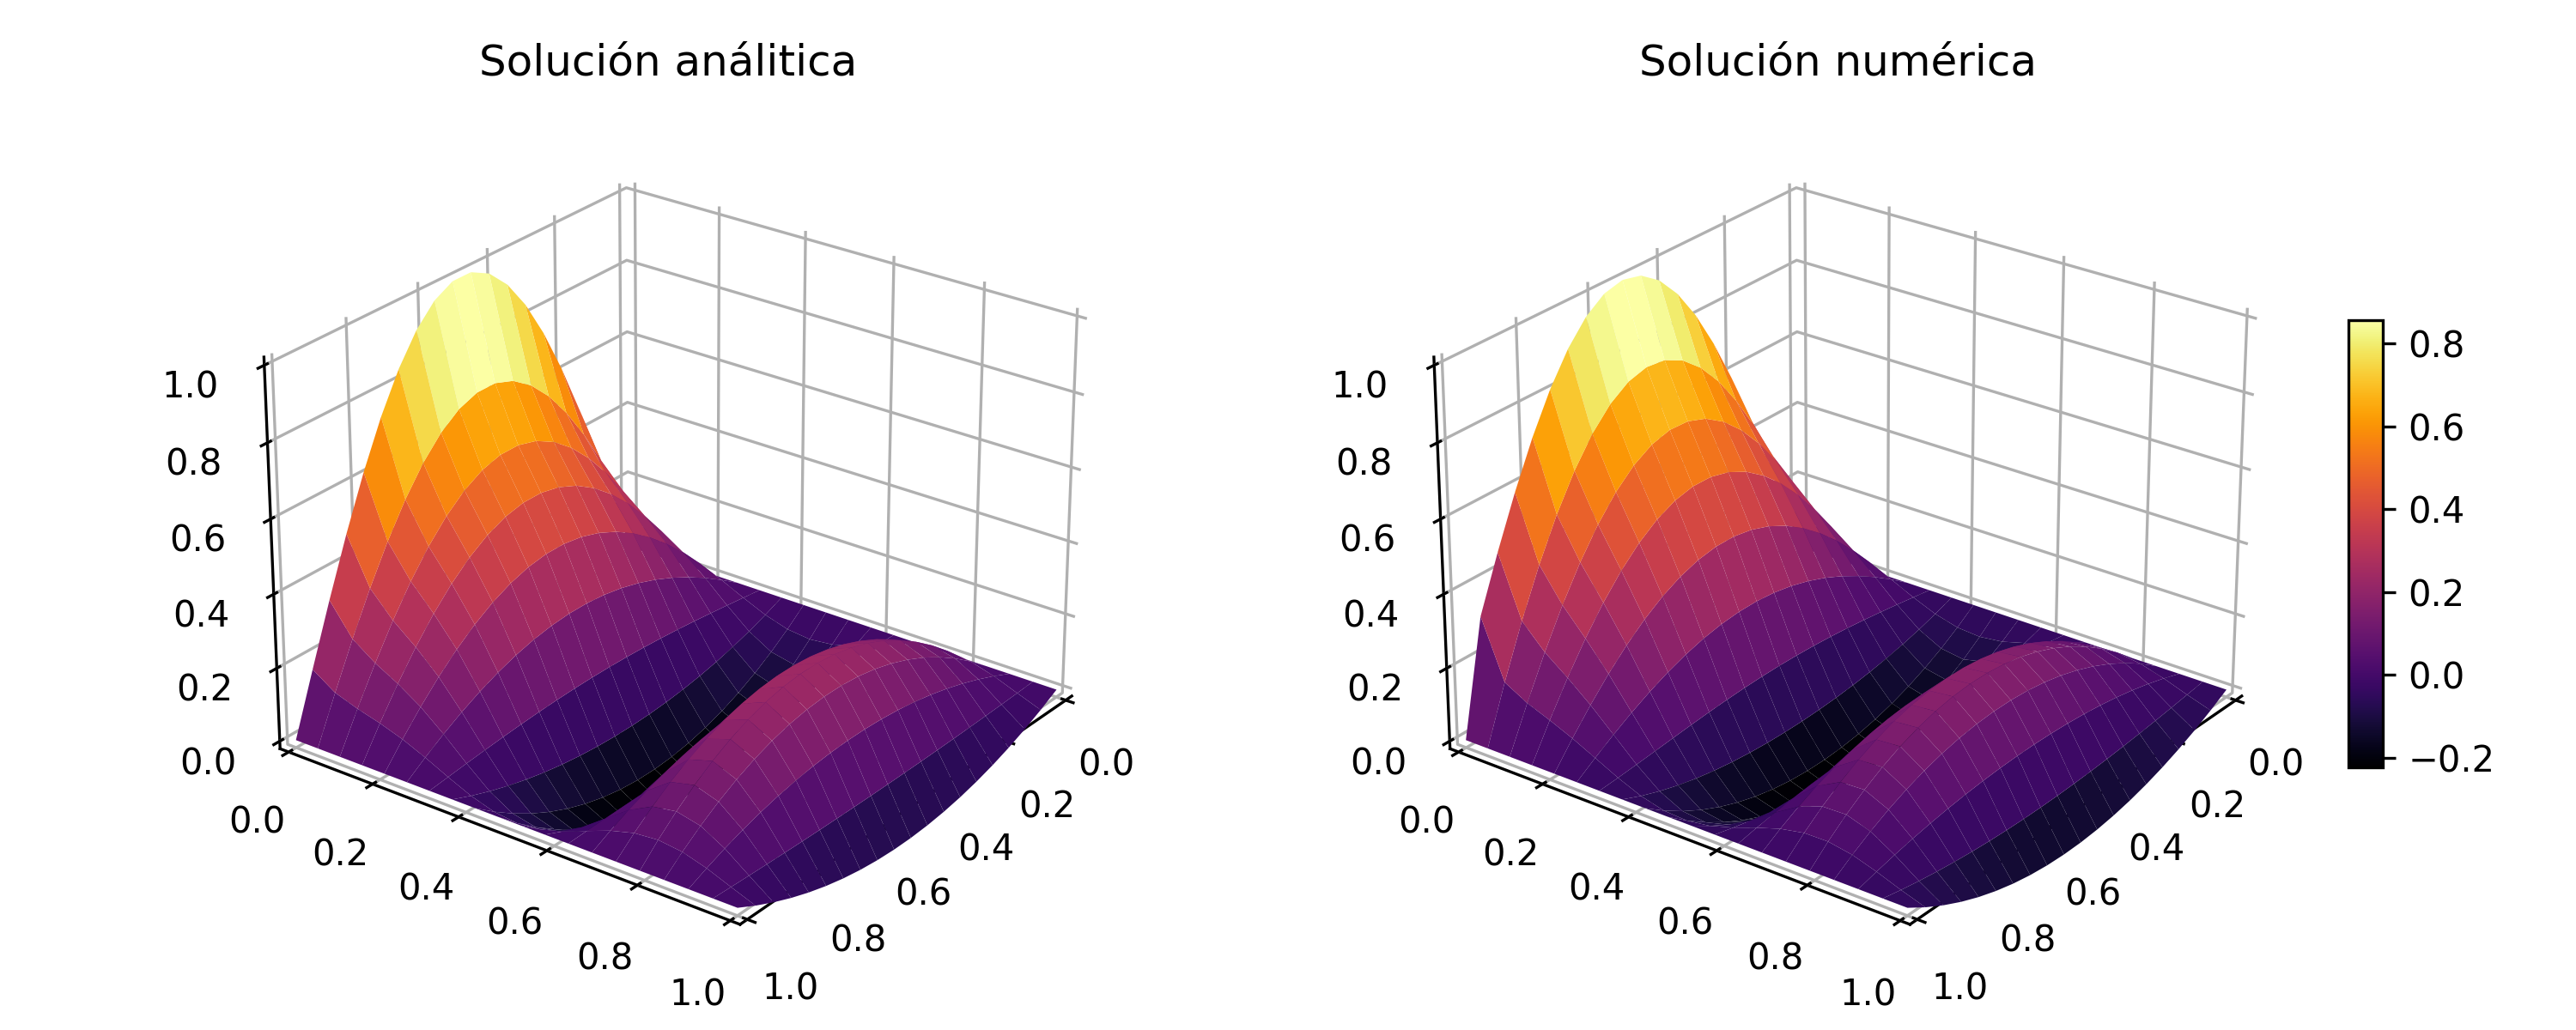
\includegraphics[width=14cm]{surface_1.png}
        \caption{\textcolor{black}{Solución de la ecuación \ref{eq:equation_1}}}
    \end{figure}
\end{frame}

\begin{frame}
    \begin{figure}
        \centering
        \includegraphics[width=5cm]{frames/01/000.png}
        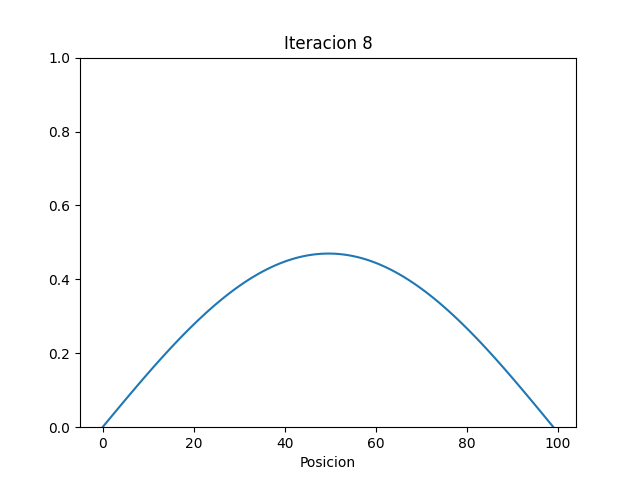
\includegraphics[width=5cm]{frames/01/008.png}
        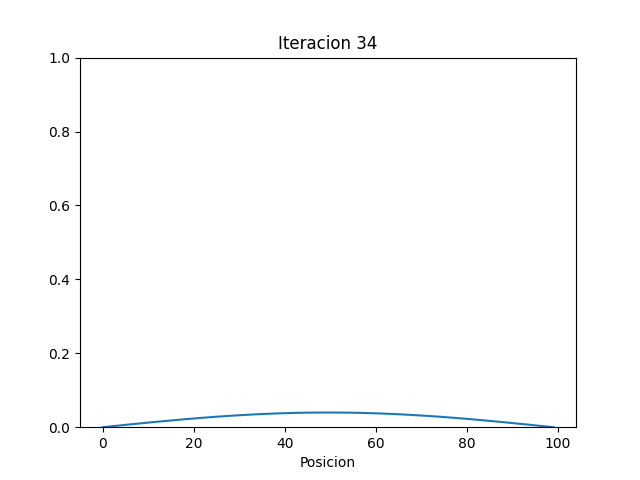
\includegraphics[width=5cm]{frames/01/034.png}
        \includegraphics[width=5cm]{frames/01/099.png}
        \caption{
            \textcolor{black}{
                Función u(x,t) para la ecuación} \ref{eq:equation_1}.}
    \end{figure}
\end{frame}

\begin{frame}
    \misc{
        Se tiene la siguiente ecuación diferencial parcial:
        \begin{equation}
            \frac{\partial u}{\partial t} = \frac{1}{\pi^2}\frac{\partial^2 u}{\partial x^2} \qquad 0<x<1, \; t>0 \label{eq:equation_2}
        \end{equation}
        con las siguientes condiciones de frontera:
        \begin{equation*}
            \begin{cases}
                u(x,0) & = sin(\pi x) \qquad 0<x<1 \\
                u(0,t) & =u(1,t) = 0, \qquad t>0
            \end{cases}
        \end{equation*}
        La solución análitica de este conjuntos de ecuaciones es:
        \begin{equation*}
            u(x,t)= e^{-t}sin(\pi x)
        \end{equation*}}
\end{frame}

\begin{frame}
    \begin{figure}[H]
        \centering
        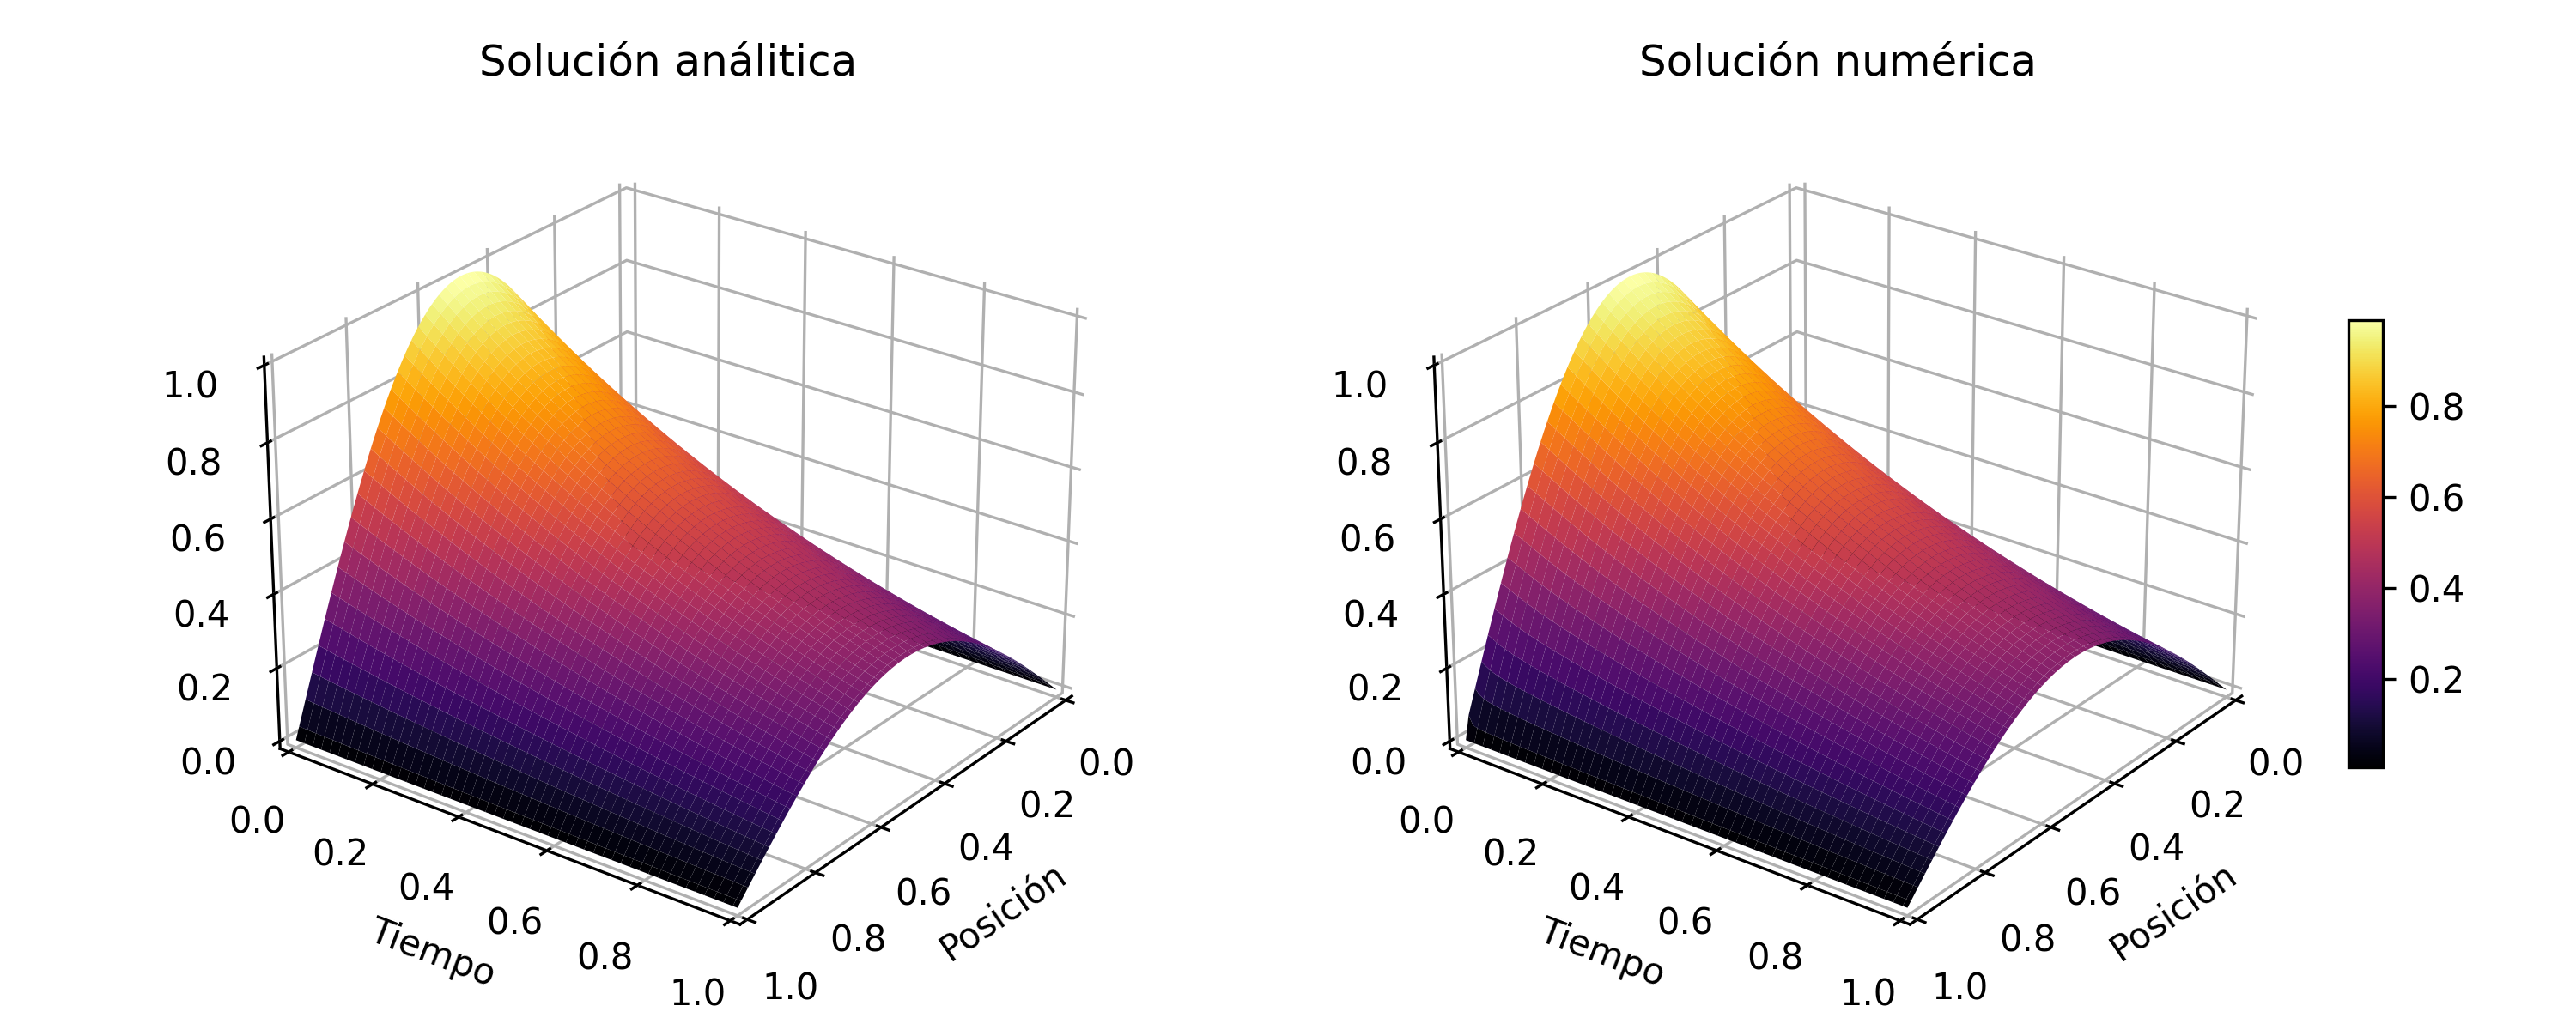
\includegraphics[width=14cm]{surface_2.png}
        \caption{\textcolor{black}{Solución de la ecuación \ref{eq:equation_2}}}
    \end{figure}
\end{frame}

\begin{frame}
    \begin{figure}
        \centering
        \includegraphics[width=5cm]{frames/02/000.png}
        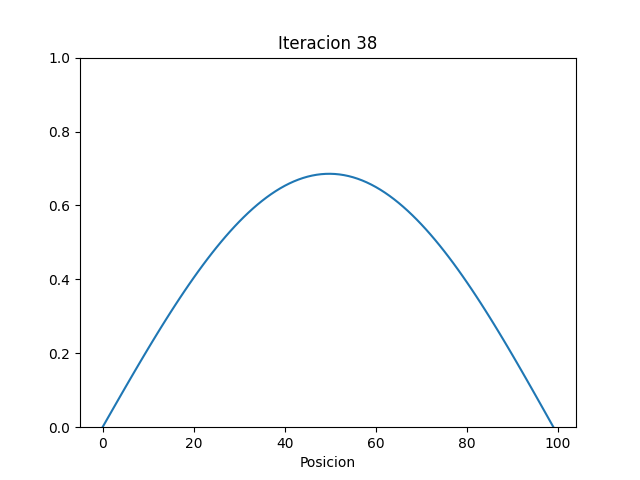
\includegraphics[width=5cm]{frames/02/038.png}
        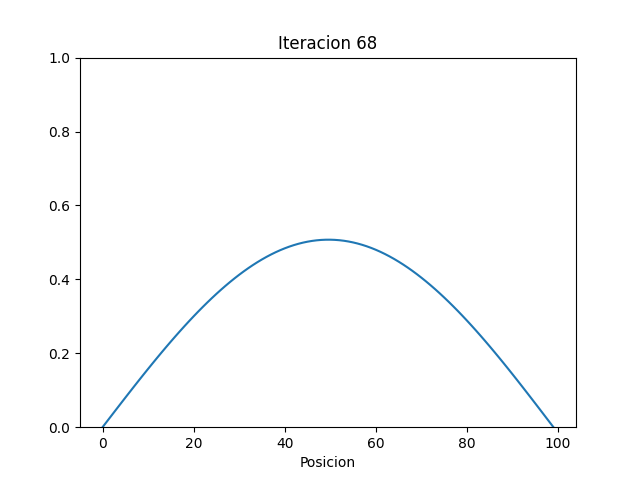
\includegraphics[width=5cm]{frames/02/068.png}
        \includegraphics[width=5cm]{frames/02/099.png}
        \caption{
            \textcolor{black}{
                Función u(x,t) para la ecuación} \ref{eq:equation_2}.}
    \end{figure}
\end{frame}

\begin{frame}
    \misc{
        Se tiene la siguiente ecuación diferencial parcial:
        \begin{equation}
            \frac{\partial u}{\partial t} = \frac{\partial^2 u}{\partial x^2}+10x(1-x)cos(10t)+2sin(10t)\qquad 0<x<1, \; t>0 \label{eq:equation_3}
        \end{equation}
        con las siguientes condiciones de frontera:
        \begin{equation*}
            \begin{cases}
                u(x,0) & = sin(\pi x) \qquad 0<x<1 \\
                u(0,t) & =u(1,t) = 0, \qquad t>0
            \end{cases}
        \end{equation*}
        La solución análitica de este conjuntos de ecuaciones es:
        \begin{equation*}
            u(x,t)= e^{-\pi^2 t}sin(\pi x)+x(1-x)sin(10t)
        \end{equation*}
    }
\end{frame}

\begin{frame}
    \begin{figure}[H]
        \centering
        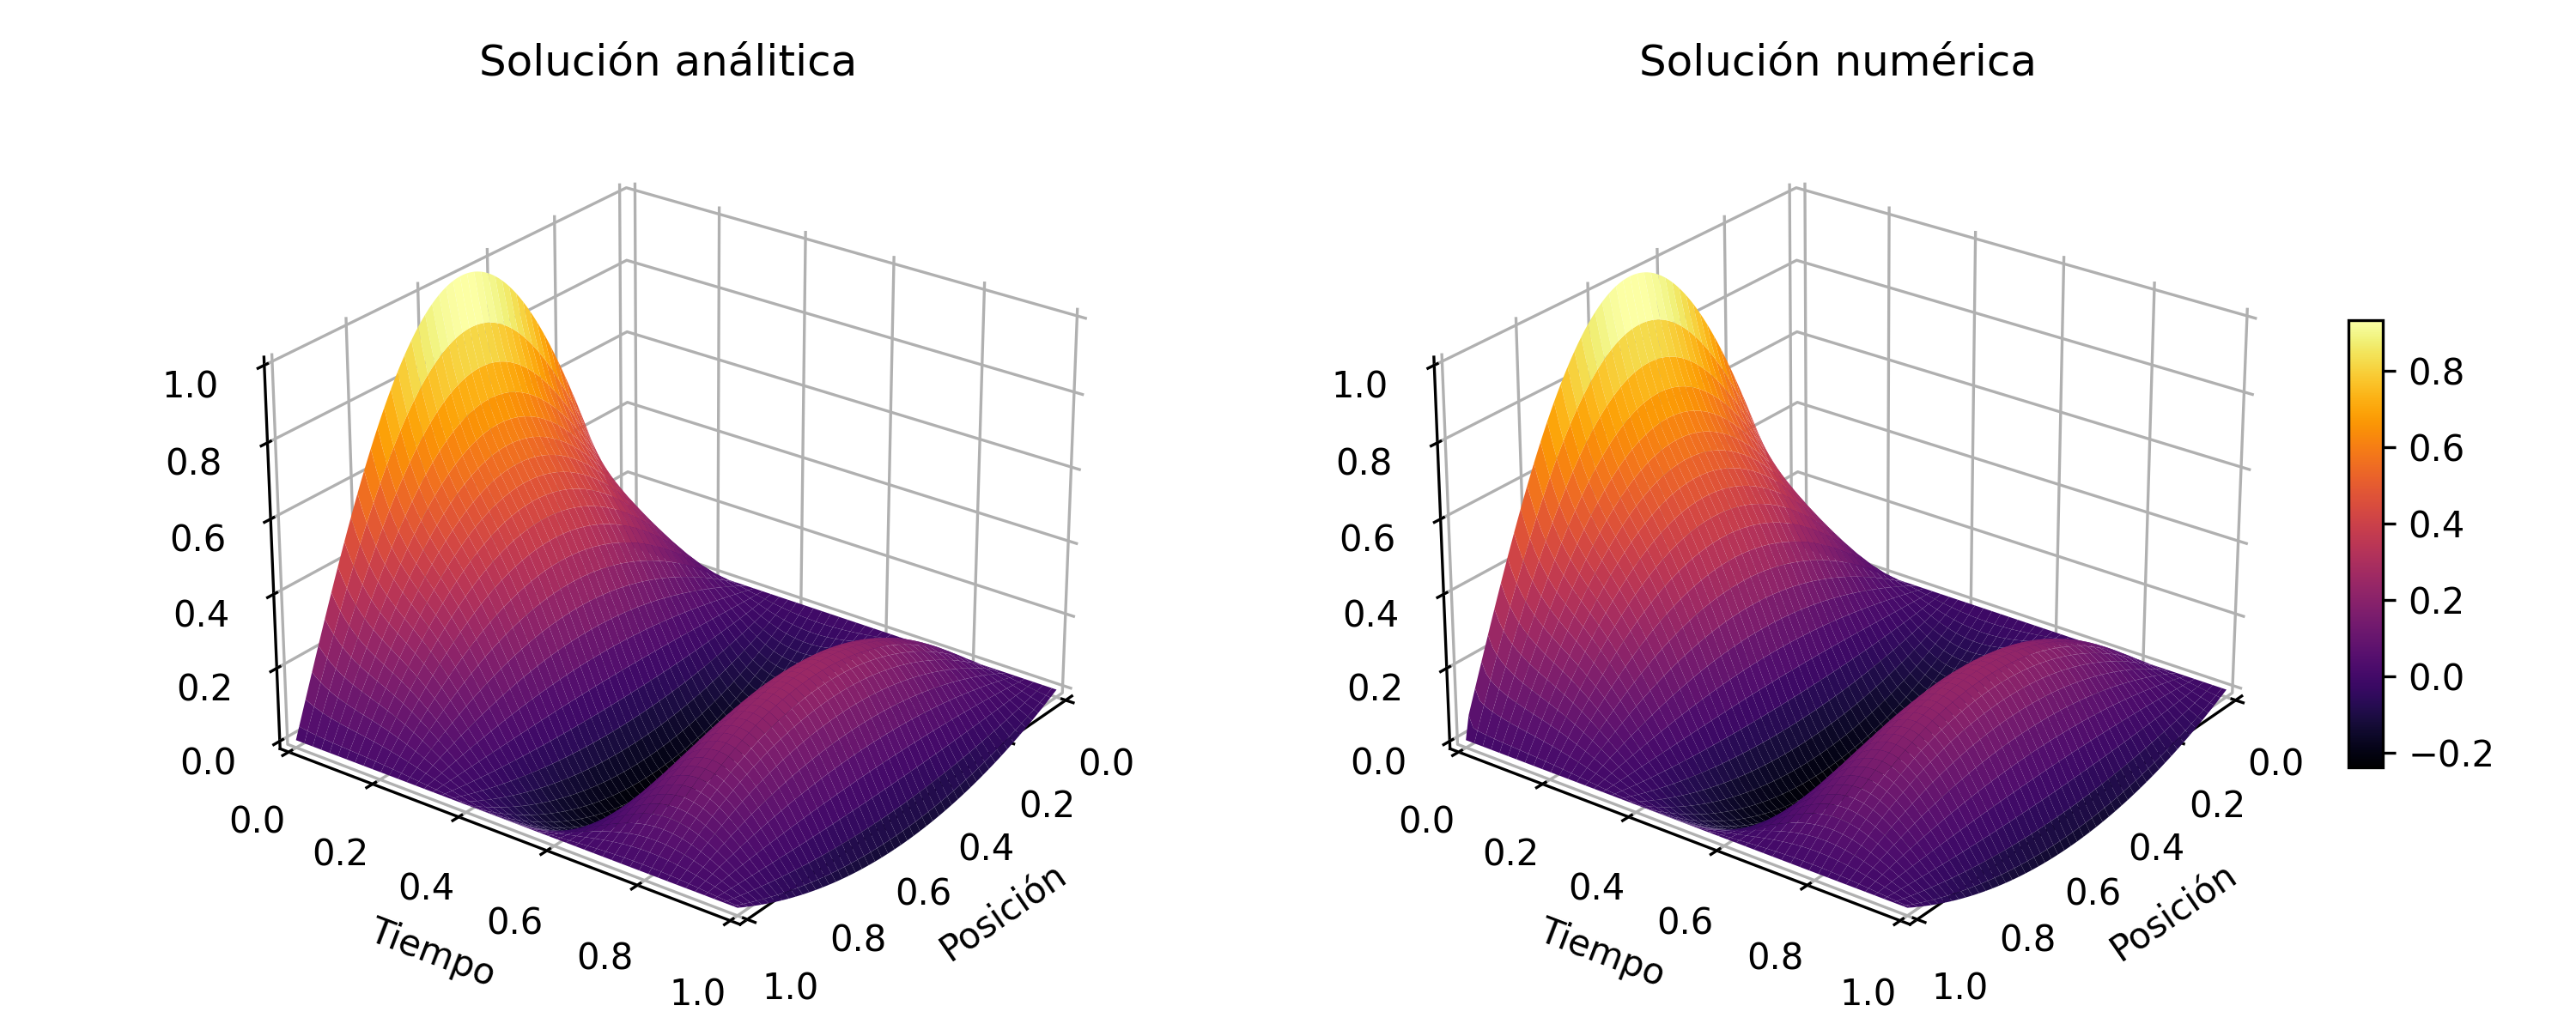
\includegraphics[width=14cm]{surface_3.png}
        \caption{\textcolor{black}{Solución de la ecuación \ref{eq:equation_3}}}
    \end{figure}
\end{frame}

\begin{frame}
    \begin{figure}
        \centering
        \includegraphics[width=5cm]{frames/03/000.png}
        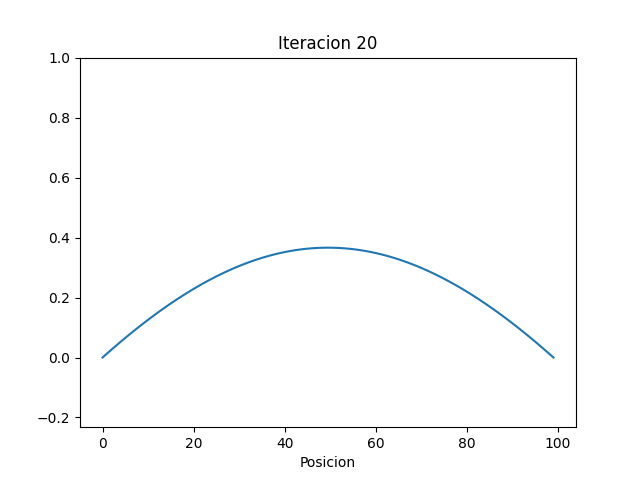
\includegraphics[width=5cm]{frames/03/020.png}
        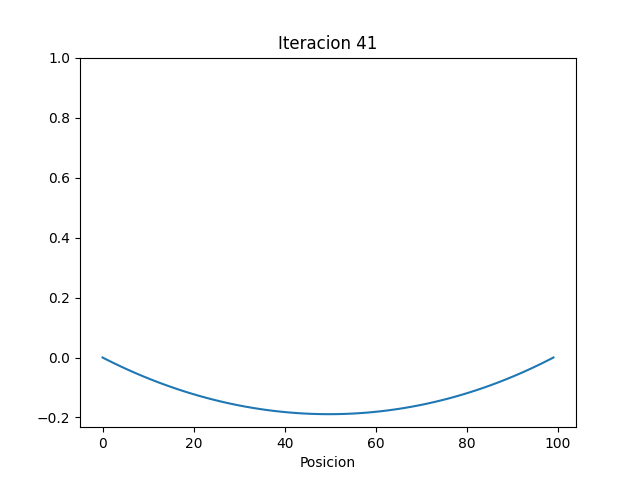
\includegraphics[width=5cm]{frames/03/041.png}
        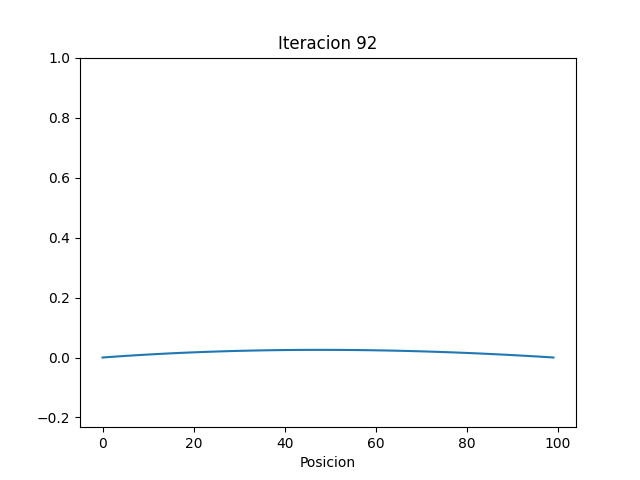
\includegraphics[width=5cm]{frames/03/092.png}
        \caption{
            \textcolor{black}{
                Función u(x,t) para la ecuación} \ref{eq:equation_3}.}
    \end{figure}
\end{frame}

\begin{frame}
    \misc{
        Se tiene la siguiente ecuación diferencial parcial:
        \begin{equation}
            \frac{\partial u}{\partial t} = 4\frac{\partial^2 u}{\partial x^2}+e^tsin(x)\qquad 0<x<\pi, \; t>0 \label{eq:equation_4}
        \end{equation}
        con las siguientes condiciones de frontera:
        \begin{equation*}
            \begin{cases}
                u(x,0) & = sin(\pi x) \qquad 0<x<1 \\
                u(0,t) & =u(\pi,t) = 0, \qquad t>0
            \end{cases}
        \end{equation*}
        La solución análitica de este conjuntos de ecuaciones es:
        \begin{equation*}
            u(x,t)=\frac{1}{5}( e^t-e^{-4t})sin(x)
        \end{equation*}}
\end{frame}

\begin{frame}
    \begin{figure}[H]
        \centering
        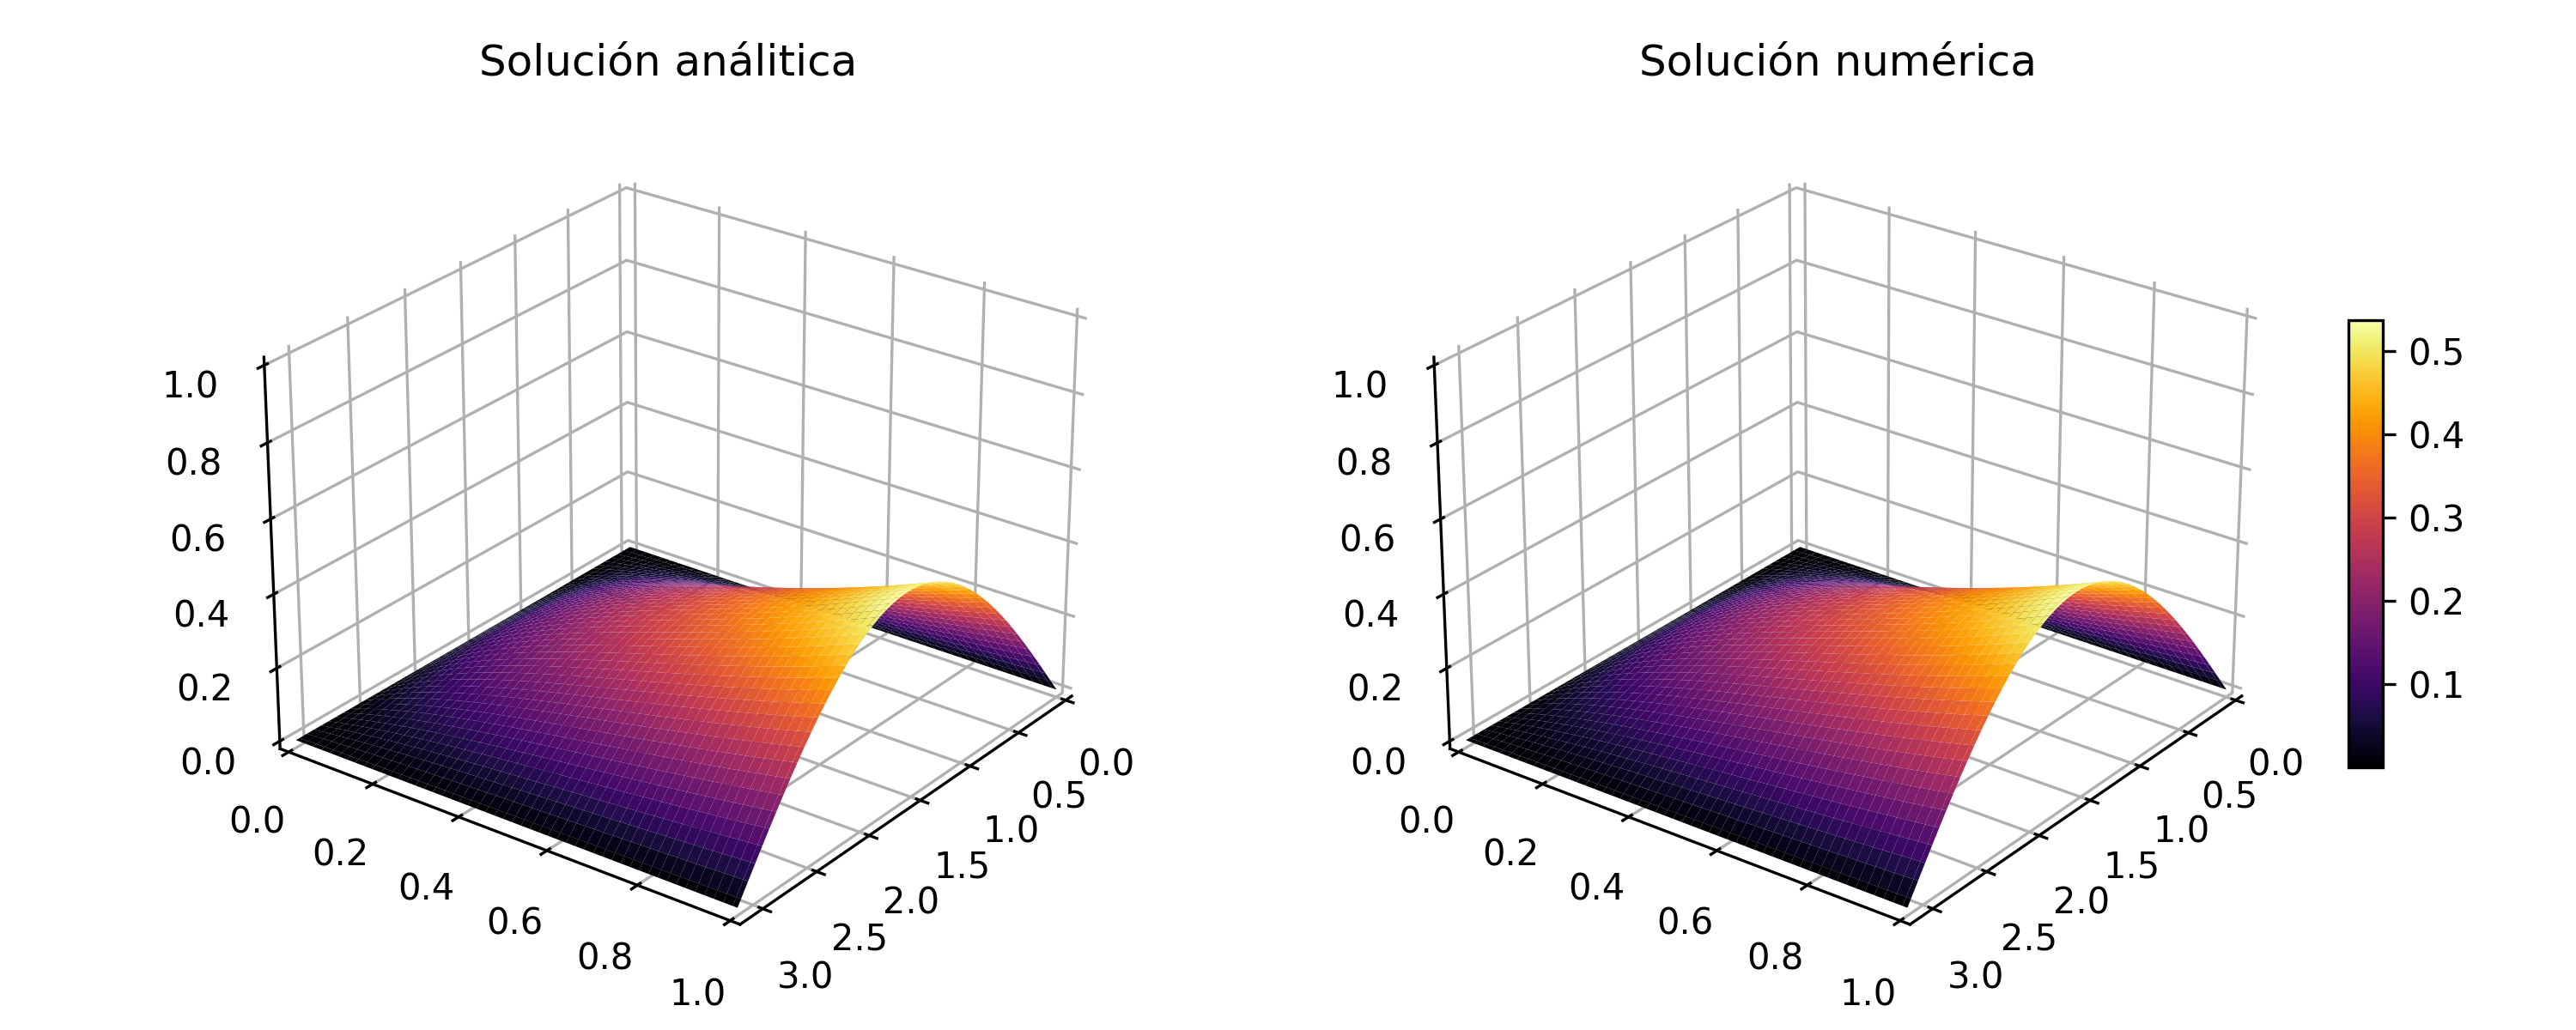
\includegraphics[width=14cm]{surface_4.png}
        \caption{\textcolor{black}{Solución de la ecuación \ref{eq:equation_4}}}
    \end{figure}
\end{frame}

\begin{frame}
    \begin{figure}
        \centering
        \includegraphics[width=5cm]{frames/04/000.png}
        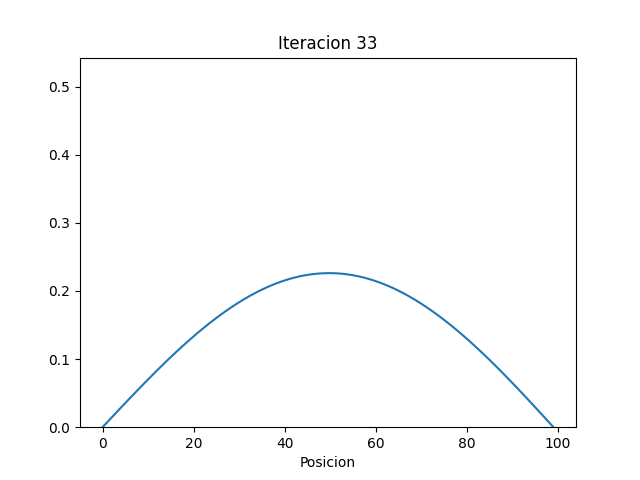
\includegraphics[width=5cm]{frames/04/033.png}
        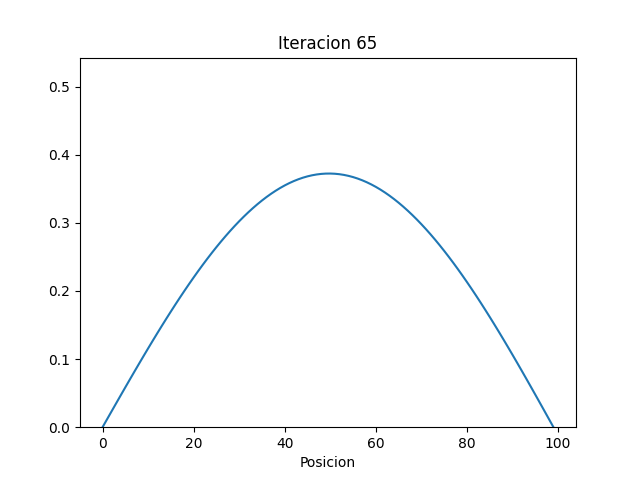
\includegraphics[width=5cm]{frames/04/065.png}
        \includegraphics[width=5cm]{frames/04/099.png}
        \caption{
            \textcolor{black}{
                Función u(x,t) para la ecuación} \ref{eq:equation_4}.}
    \end{figure}
\end{frame}

\begin{frame}
    \misc{
        \begin{table}[H]
            \centering
            \begin{tabular}{cc} \hline
                \textbf{Ecuación diferencial parcial} & \textbf{Diferencia absoluta relativa promedio} \\ \hline
                Ecuación \ref{eq:equation_1}          & 0.3531\%                                       \\
                Ecuación \ref{eq:equation_2}          & 0.3512\%                                       \\
                Ecuación \ref{eq:equation_3}          & 0.4409\%                                       \\
                Ecuación \ref{eq:equation_4}          & 0.0997\%
                \\ \hline
            \end{tabular}
            \caption{Diferencias absolutas promedio de los resultados numéricos con respecto a la solución análitica.}
        \end{table}

    }
\end{frame}